\documentclass[12pt,a4paper]{report}
%\linespread{1.3}
\usepackage{fullpage}
\usepackage{setspace}
\usepackage[margin = 1in, left = 1.3in]{geometry} %to change margin dimension
\usepackage{xcolor}
\usepackage{hyperref}
\usepackage{url}
\usepackage{pifont,multirow}
\usepackage{enumitem}
\usepackage{graphics,graphicx,url, wrapfig,latexsym,epsfig}
\usepackage{hyperref,comment,epic}
\usepackage{amsmath,algorithm}
\usepackage{algpseudocode}
\usepackage{makeidx,setspace}
\usepackage{longtable}
\usepackage{mdwmath,mdwtab}
\usepackage{stfloats}
\usepackage{subfig}
\usepackage{verbatim}
\usepackage[titletoc]{appendix}
\usepackage[stable]{footmisc}
%---------------------------------------------------------------------
\font\en="Latin Modern Roman Unslanted:script=roman" at 12pt
\font\ens="Latin Modern Roman Unslanted:script=roman" at 12pt
%----------------------------------------------------------------------
\graphicspath{{figures/}}
\setlength{\parskip}{1mm}
\setlength{\lineskip}{1mm}
\setlength{\parindent}{20pt}
\hypersetup{
    bookmarks=true,         % show bookmarks bar?
    unicode=true,          % non-Latin characters in Acrobat’s bookmarks
    pdftoolbar=true,        % show Acrobat’s toolbar?
    pdfmenubar=true,        % show Acrobat’s menu?
    pdfauthor={IIITM},     % author
    colorlinks=true,       % false: boxed links; true: colored links
    linkcolor= blue,          % color of internal links
    citecolor=magenta,        % color of links to bibliography
    filecolor=cyan,      % color of file links
    urlcolor=magenta           % color of external links
}
%-------------------------------------------------------------------
\newcommand{\FF}{\vspace*{\medskipamount}}
\newcommand{\act}[1]{\mbox{#1}}
\newcommand{\sglspc}{\renewcommand{\baselinestretch}{1.00}\normalsize}
\newcommand*\circled[1]{\tikz[baseline=(char.base)]{%
            \node[shape=circle,draw,inner sep=1pt] (char) {#1};}}

\makeatletter
\newenvironment{tablehere}{\def\@captype{table}}{}
\newenvironment{figurehere} {\def\@captype{figure}}{}
\makeatother

\newcommand{\newphases}{\setcounter{phase}{0}}
\newcommand{\phase}[1]{\vspace{1 ex}\addtocounter{phase}{1}\par\noindent{\bf \Alph{phase} #1}}
\newcommand{\phaselabel}[1]{\newsavebox{#1}\sbox{#1}[\Alph{phase}]}
\newcommand{\phaseref}[1]{\usebox{#1}}
%++++++++++++++++++++++++++++++++++++++++++++++++++++++++++
\makeindex
\newcolumntype{L}{>{\arraybackslash}m{5.7cm}}
\newcolumntype{T}{>{\arraybackslash}m{2.3cm}}
%++++++++++++++++++++++++++++++++++++++++++++++++++++++++++
\usepackage{listings}
\usepackage{color}

\definecolor{dkgreen}{rgb}{0,0.6,0}
\definecolor{gray}{rgb}{0.5,0.5,0.5}
\definecolor{mauve}{rgb}{0.58,0,0.82}

\lstset{frame=tb,
  language=Matlab,
  aboveskip=3mm,
  belowskip=3mm,
  showstringspaces=false,
  columns=flexible,
  basicstyle={\small\ttfamily},
  numbers=none,
  numberstyle=\tiny\color{gray},
  keywordstyle=\color{blue},
  commentstyle=\color{dkgreen},
  stringstyle=\color{mauve},
  breaklines=true,
  breakatwhitespace=true,
  tabsize=3
}
%++++++++++++++++++++++++++++++++++++++++++++++++++++++++++

\begin{document}
\pagenumbering{roman}
\thispagestyle{empty}
\begin{center}

\vspace*{0.7 cm}
\begin{center}
	\begin{center}
	\color{lightgray}
		\line(1,0){450}\\
	\end{center}
	\vspace{0.3 in}
	{\huge{\bf End-Semester Assignment}}
	\begin{center}
		\color{lightgray}
		\line(1,0){250}\\
	\end{center}
\end{center}
{\en To - Dr Subasit Borah (Ph D)}

By
			       
{\Large \bf Aman Ranjan Verma\\}
{\en Bachelor of Technology, VIII Semester\\}
{\en 15010212}\\

\vspace{1.5 in}
\vspace{0.8 in}

\includegraphics[scale=0.95]{iiitm-logo.png}
\vspace{0.8 in}

{\large\bf Department of Electronics and Communication Engineering\\}
\textsc{\large\bf Indian Institute of Information Technology\\ Senapati, Manipur}\\
%{\large\bf Imphal, India - 795002\\}
{\large 10 Apr, 2019 }

\end{center}


\cleardoublepage\phantomsection
\setcounter{secnumdepth}{4}
\setcounter{tocdepth}{4}
\pagenumbering{arabic}
\setcounter{page}{0}

\chapter{Solutions}\label{chap1}

\section{Q1.} %+++++++++++++++++++++++++++++++++++++
Solution:\\

Given,

$Z_L = 100 \Omega$

$Z_{in} = 50 \Omega$

Also we know that for $\frac{\lambda}{4}$ transmission line characteristic impedance is given by,

\begin{align*} 
Z_o & = \sqrt{Z_L Z_{in}}\\
=> Z_o &= \sqrt{100*50}\\
=> Z_o &= 70.71 \Omega
\end{align*}

Now, The reflection coefficient is given by equation,

$$ \left| \tau \right| = \left| \frac{Z_o - Z{in}}{Z_o + Z{in}}\right|$$

Where, $Z_{in}$ is frequency dependent and is given by equation,
$$Z_{in}(z = -l) = Z_o\frac{Z_L+jZ_o tan(\beta l)}{Z_o+jZ_L tan(\beta l)}$$

Therefore, the equation for $\tau$ is also frequency dependent$(f)$, since
$$\beta l = \pi/2 \frac{f}{f_o}$$

\newpage
The plot for reflection coefficient ($\tau$) Vs $\frac{f}{f_o}$ is shown in figure \ref{q1}:
\begin{figure}[!ht]
	\centering
	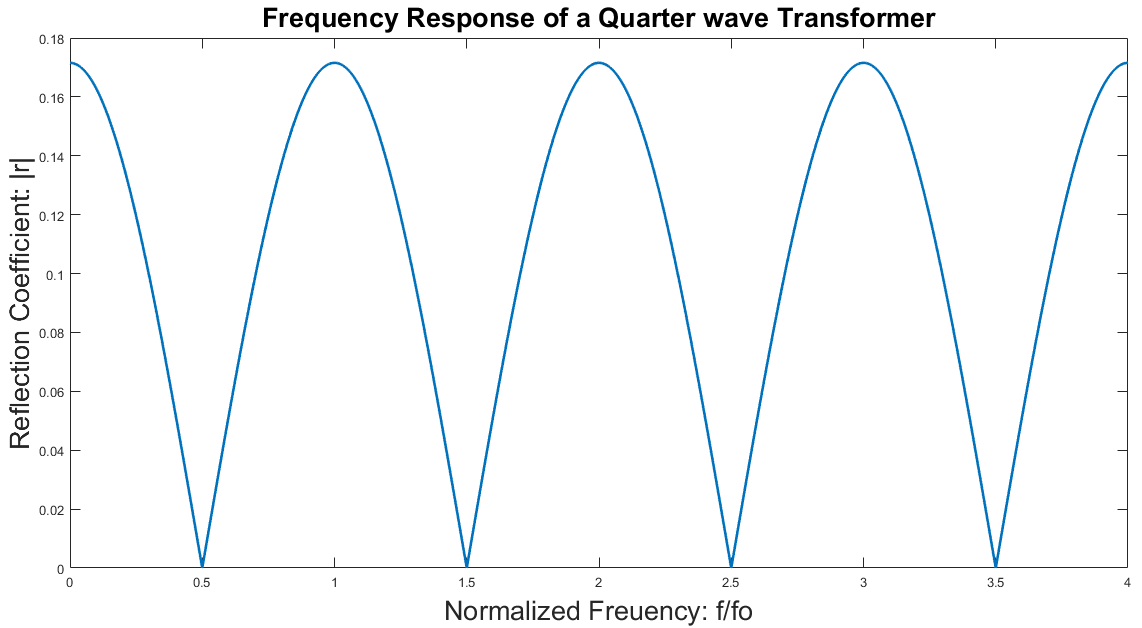
\includegraphics[scale=0.45]{q1.png}
	\caption{\label{q1} Reflection Coefficient Vs Normalized Frequency}
\end{figure}

Matlab Code
\begin{lstlisting}
f_fo = 0:0.01:4; % f_fo represents normalised frequency f/fo
Bl = pi*f_fo/2; % Bl represents B*l
zo = 70.71; % Charecteristic Impedance
zl = 100; % Load Impedance
zin = abs(zo*(zl + 1i*zo*tan(Bl))./(zo + 1i*zl*tan(Bl))); %Input Impedance
tau = (zo - zin)./(zo + zin); % Reflection Coefficient
plot(f_fo, abs(tau), 'LineWidth',2)
title('Frequency Response of a Quarter wave Transformer', 'FontSize', 15)
xlabel('Normalized Freuency: f/fo', 'FontSize',12)
ylabel('Reflection Coefficient: |r|', 'FontSize',12)
\end{lstlisting}


\section{Q2.} %+++++++++++++++++++++++++++++++++++++
Solution:\\

Standing wave is superposition of incident wave and reflected wave \cite{link1}. Let incident wave be represented by $V_i$ and reflected wave be represented by $V_r$.
\begin{align*} 
V_i &= Sin(x), \;\;\;\; Assumption  \\
So, V_r &= \tau Sin(x + \pi)
\end{align*}

$V_r$ is a $\pi$ angle phase shift of $Vi$ multiplied by reflection coefficient $\tau.$ Phase shift by $\pi$ is as per the reflection property of wave \cite{link2}. 

Standing wave pattern for $\tau = 0.1$ and $\tau = 1$ are:
\begin{figure}[!ht]
	\centering
	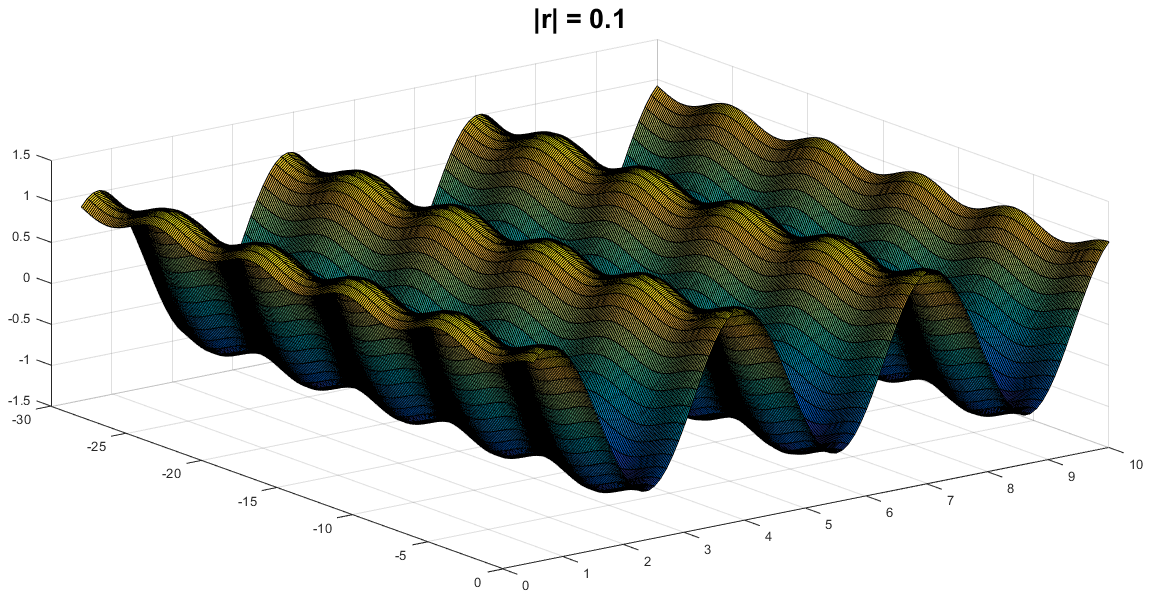
\includegraphics[scale=0.45]{q2a.png}
	\caption{\label{q1} Standing wave pattern for $\tau = 0.1$}
\end{figure}

\newpage
Matlab Code
\begin{lstlisting}
tau = 0.1; % Reflection Coefficient
[X,Y] = meshgrid(0:0.1:30, 0.5:0.1:10); % Axix range
Z = sin(2*Y) - tau*sin(1*X); % Standing Wave (Superposition)
surf(-X, Y, Z) % 3D Plot Function 
title('|r| = 1', 'FontSize', 20)
\end{lstlisting}


\begin{figure}[!ht]
	\centering
	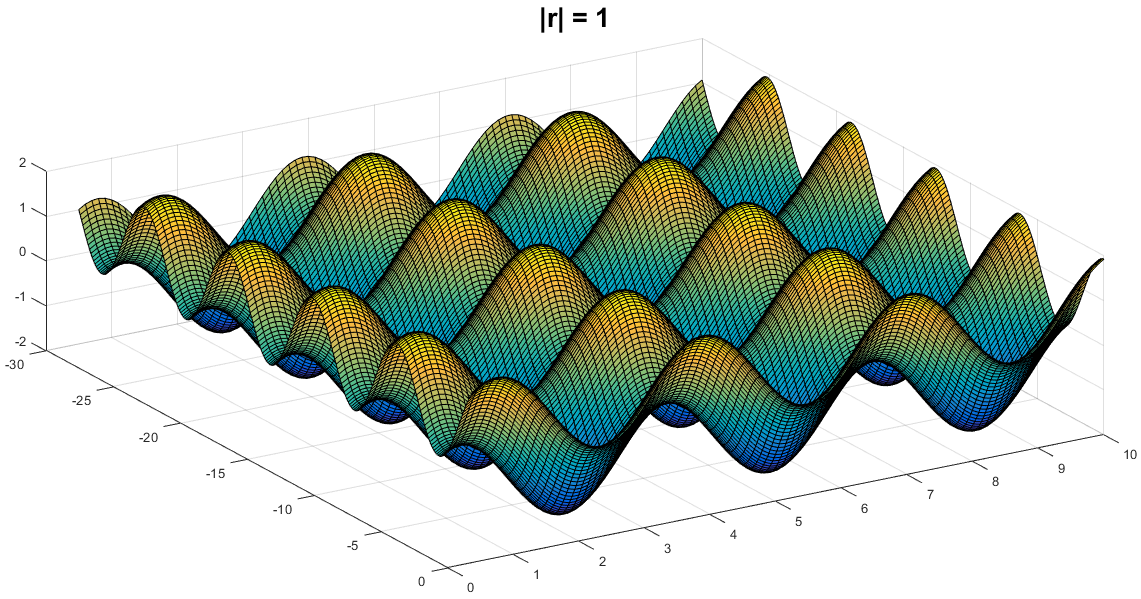
\includegraphics[scale=0.45]{q2b.png}
	\caption{\label{q1}  Standing wave pattern for $\tau = 1$}
\end{figure}

Matlab Code
\begin{lstlisting}
tau = 1; % Reflection Coefficient
[X,Y] = meshgrid(0:0.1:30, 0.5:0.1:10); % Axis range
Z = sin(2*Y) - tau*sin(1*X); % Standing Wave (Superposition)
surf(-X, Y, Z) % 3D Plot Function 
title('|r| = 1', 'FontSize', 20)
\end{lstlisting}

   
\section{Q3.} %++++++++++++++++++++++++++++
Solution:\\

Input impedance of a transmission line is given by equation:
$$Z_{in}(z = -l) = Z_o\frac{Z_L + j Z_o tan(\beta l)}{Z_o + j Z_L tan(\beta l)}$$

For a transmission line that is terminated in a short circuit, the equation decomposes to:
$$ Z_{in}(z = -l) = j Z_o tan(\beta l)$$

Matlab Code to compute input impedance when $2 \beta l$ is passed as input.
\begin{lstlisting}
two_Bl = input('Enter value for 2Bl: ');
Bl = two_Bl/2;
zo = 1; % Charecteristic Impedance
zl = 0; % Load Impedance
zin = 1i*zo*tan(Bl); %Input Impedance
display('Input Impedance is:')
display(zin)
\end{lstlisting}

OUTPUT
\begin{figure}[!ht]
	\centering
	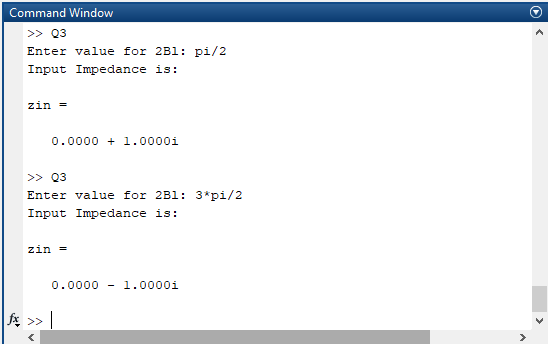
\includegraphics[scale=0.9]{q3.png}
	\caption{\label{q1}  Input Impedance for $2 \beta l = \{90', 270'\}$}
\end{figure}

\newpage
\section{Q4.} %++++++++++++++++++++++++++++
\subsection{a}
Solution:\\

The coupler shown in figure \ref{front}, \ref{cross}, \ref{rad_box} is designed in HFSS software. Design parameters assumed in the designing the coupler are as per the question description. Apart from that other assumptions are:

\begin{itemize}
		\item Substrate: "Rogers Ultralam 2000 (tm)"
		\item Shape and size of the coupler \cite{4084811}.
\end{itemize}

\begin{figure}[!htb]
   \begin{minipage}{0.48\textwidth}
     \centering
     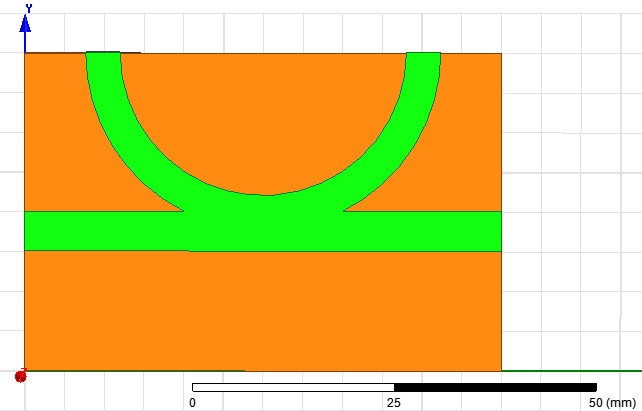
\includegraphics[scale=0.45]{front.png}
     \caption{Front view of coupler}\label{front}
   \end{minipage}
   \begin{minipage}{0.48\textwidth}
     \centering
     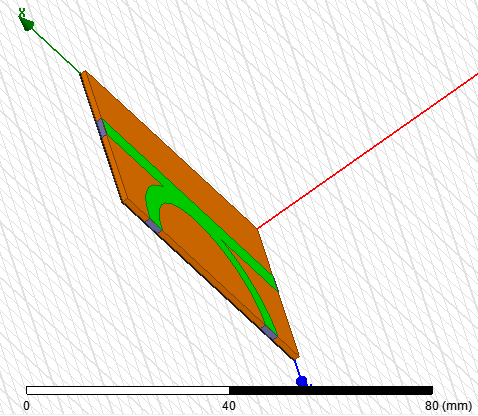
\includegraphics[scale=0.45]{cross.png}
     \caption{Cross Sectional View of coupler}\label{cross}
   \end{minipage}
\end{figure}

\begin{figure}[!ht]
	\centering
       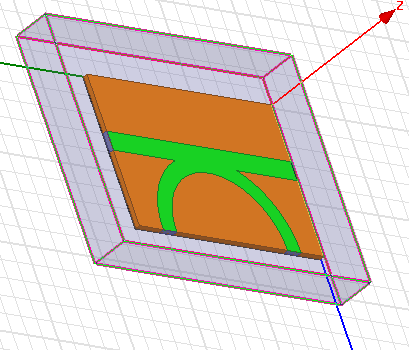
\includegraphics[scale=0.45]{rad_box.png}
       \caption{Coupler with radiation box}\label{rad_box}
\end{figure}

S-Matrix is shown in table \ref{sm} at frequency = 3GHz when port 1 i s excited.
\begin{table}[!ht]
\centering
\begin{footnotesize}
\begin{tabular}{ |cccc|c|cccc|  }
S11 & S12 & S13 & S14 & & -11.33074065 & -3.01406265 & -12.07898315 & -10.31970471\\
S21 & S22 & S23 & S24 &=& 0 & 0 & 0 & 0 \\
S31 & S32 & S33 & S34 & & 0 & 0 & 0 & 0 \\
S41 & S42 & S43 & S44 & & 0 & 0 & 0 & 0 \\
\end{tabular}
\end{footnotesize}
\caption{\label{sm} S-Matrix}
\end{table}

Similarly, the values for other $S_{mn}$ are calculated by exciting other ports.

\newpage
Matlab Code to plot the S-Parameter,
\begin{lstlisting}
filename = 'coupler.csv'; % S-Parameter values are extracted from HFSS into coupler.csv
M = csvread(filename, 1, 0);
t = 1:5:601;
plot(M(t, 1), M(t, 2), 'b-+', 'LineWidth', 1) % Plot for S11
hold on 
plot(M(t, 1), M(t, 3), 'g-', 'LineWidth', 1) % Plot for S12
hold on
plot(M(t, 1), M(t, 4), 'm-o', 'LineWidth', 1) % Plot for S13
hold on 
plot(M(t, 1), M(t, 5), 'r-*', 'LineWidth', 1) % Plot for S14
legend('S11:Input', 'S12:Through', 'S13:Coupled', 'S14:Isolation')
axis([0 6 -50 0])
grid on;
text(2.5, -11.3, '3 GHz, -12 db', 'Color', 'black','FontSize',10)
title('Scattering Matrix Plot', 'FontSize', 20)
xlabel('Freuency (GHz)', 'FontSize', 20)
ylabel('S Parameter', 'FontSize', 20)
\end{lstlisting}


OUTPUT
\begin{figure}[!ht]
	\centering
	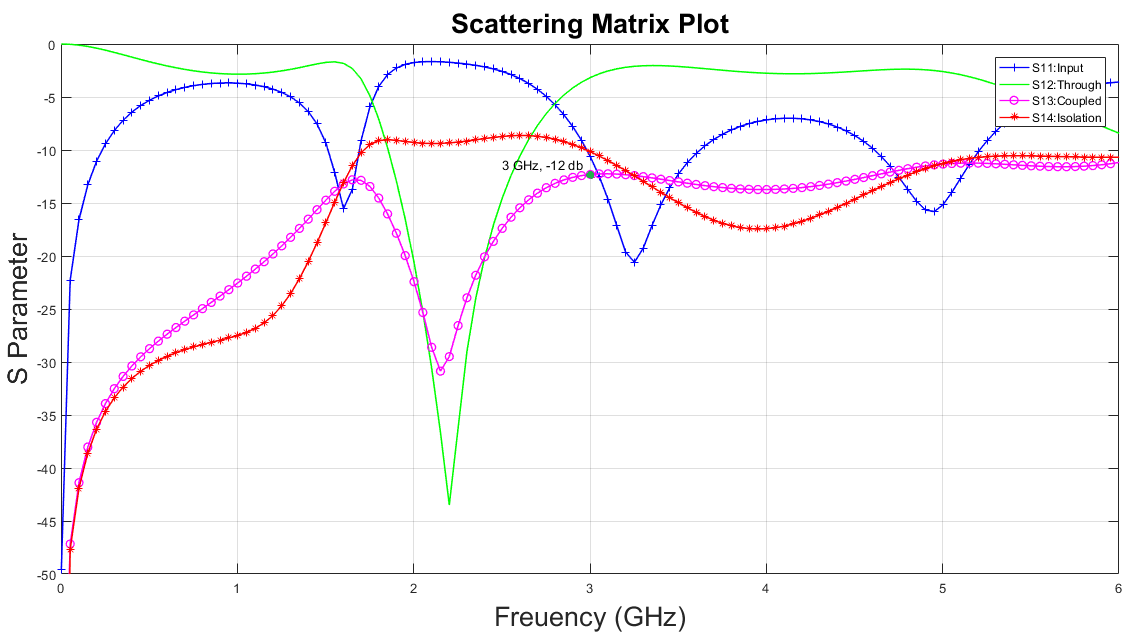
\includegraphics[scale=0.55]{s_matrix.png}
	\caption{\label{s_matrix} S-Parameter plot}
\end{figure}

\newpage
Matlab Code to plot the $|S|^2$-Parameter,
\begin{lstlisting}
filename = 'coupler.csv'; % S-Parameter values are extracted from HFSS into coupler.csv
M = csvread(filename, 1, 0);
t = 1:5:601;
plot(M(t, 1), 10*log10((10.^(M(t, 2)./10)).^2), 'b-+', 'LineWidth', 1) % Plot for |S11|^2
hold on 
plot(M(t, 1), 10*log10((10.^(M(t, 3)./10)).^2), 'g-', 'LineWidth', 1) % Plot for |S12|^2
hold on
plot(M(t, 1), 10*log10((10.^(M(t, 4)./10)).^2), 'm-o', 'LineWidth', 1) % Plot for |S13|^2
hold on 
plot(M(t, 1), 10*log10((10.^(M(t, 5)./10)).^2), 'r-*', 'LineWidth', 1) % Plot for |S14|^2
legend('S11:Input', 'S12:Through', 'S13:Coupled', 'S14:Isolation')
axis([0 6 -50 0])
grid on;
text(2.5, -11.3, '3 GHz, -12 db', 'Color', 'black','FontSize',10)
title('Scattering Matrix Plot', 'FontSize', 20)
xlabel('Freuency (GHz)', 'FontSize', 20)
ylabel('S Parameter', 'FontSize', 20)
\end{lstlisting}
OUTPUT
\begin{figure}[!ht]
	\centering
	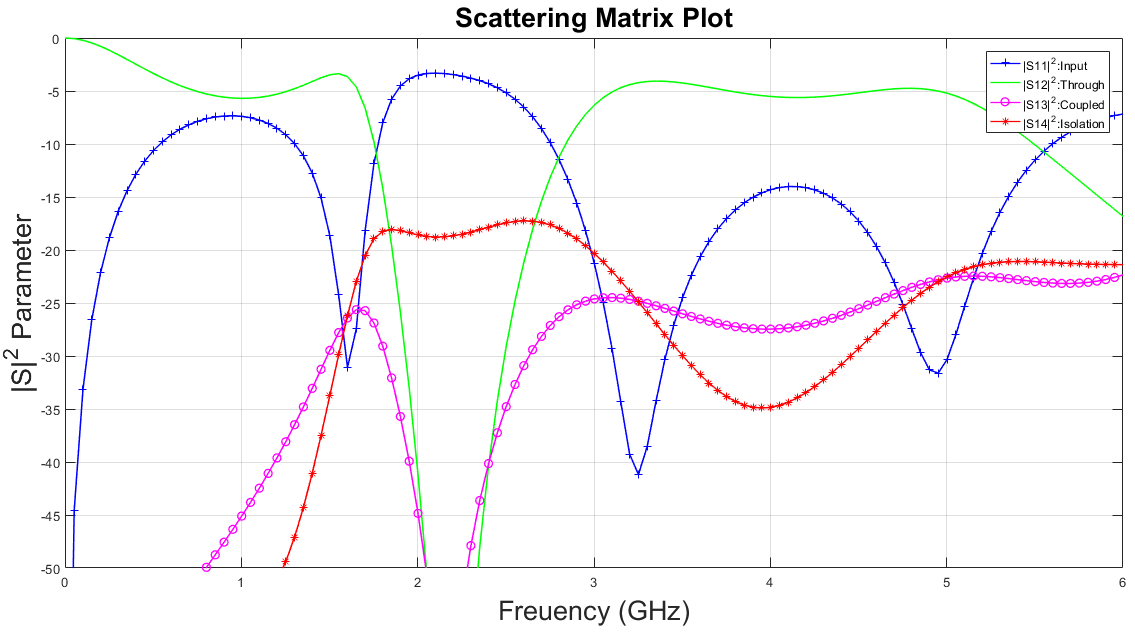
\includegraphics[scale=0.55]{s2.png}
	\caption{\label{s_matrix} $|S|^2$-Parameter plot}
\end{figure}


\subsection{b}
Solution:\\
Step by step procedure to plot signal flow graph \cite{link3} is shown in figure \ref{1}, \ref{2} and \ref{3}.

\begin{figure}[!ht]
	\centering
	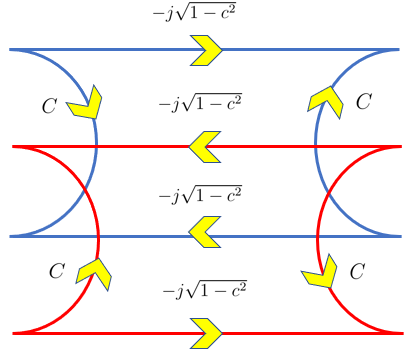
\includegraphics[scale=0.55]{1.png}
	\caption{\label{1} Step-1}
\end{figure}

\begin{figure}[!ht]
	\centering
	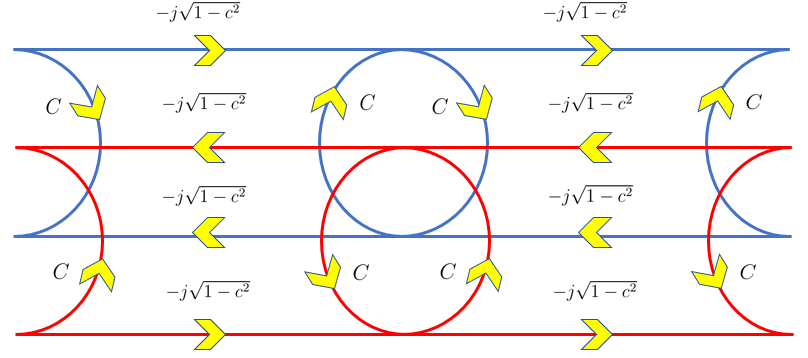
\includegraphics[scale=0.55]{2.png}
	\caption{\label{2} Step-2}
\end{figure}

\begin{figure}[!ht]
	\centering
	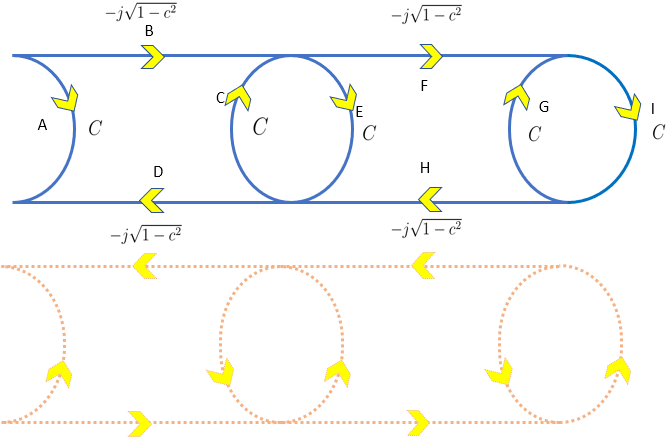
\includegraphics[scale=0.55]{3.png}
	\caption{\label{3} Step-3}
\end{figure}

Signal Flow Path = A, BED, BFIHD …..



%The goal of speech recognition is to generate the optimal word sequence subject to linguistic constraints. The sentence is composed of linguistic units such as words, syllables, phonemes. The acoustic evidence provided by the acoustic models of such units is combined with the rules to construct valid and meaningful sentences in the language. Therefore, in case of speech recognition,the pattern matching stage can be viewed as taking place in two domains: acoustic and symbolic. In the acoustic domain, a feature vector corresponding to a small segment of test speech (called a frame of speech) is matched with the acoustic model of each and every class. The segment is assigned a set of well matching class labels along with their matching scores. This process of label assignment is repeated for every feature vector in the feature vector sequence computed from the test data. The resultant lattice is processed in conjunction with the language model to yield the recognized sentence.~\cite{link4}
%
%% --------------------------------------------------------------- Speaker Recognition ---------------------------
%\section{Speaker Recognition}  Speaker recognition is the identification of a person from characteristics of voices. Speaker verification contrasts with identification. Recognizing the speaker can simplify the task of translating speech in systems that have been trained on specific voices or it can be used to authenticate or verify the identity of a speaker as part of a security process.
%
%There are two major applications of speaker recognition technologies and methodologies. If the speaker claims to be of a certain identity and the voice is used to verify this claim, this is called verification or authentication. On the other hand, identification is the task of determining an unknown speaker's identity. In a sense, speaker verification is a 1:1 match where one speaker's voice is matched to a particular template whereas speaker identification is a 1:N match where the voice is compared against a certain amount of templates. This project is related to the 1:N match type i.e., speaker identification. \\\\Speaker recognition is of two types:
%\begin{itemize}
%	\item{\bf Text-Dependent}: If the text must be the same for enrollment and verification this is called text-dependent recognition.
%	\item{\bf Text-Independent}: In this case the text during enrollment and test is different. As text-independent technologies do not compare what was said at enrollment and verification. In this project we aim at developing a text independent identification system. 
%\end{itemize}
%
%% --------------------------------------------------------------- Literature Survey ---------------------------
%\section{Literature Survey}
%Jianliang Meng Et al.~\cite{meng2012overview} states that the speech recognition system is essentially a pattern recognition system, including feature extraction, pattern matching and the reference model library. Anjali Garg Et al,~\cite{garg2016survey} states that initially, ASR systems were established on two acoustic models {\bf1.} Word model, where the size of vocabulary is small and the word is modeled as a whole and {\bf2.} Phone model, where only parts of words i.e., phonemes are modeled. 
%
%Usha Sharma Et al,~\cite{7154944} discuss all traditionally used feature extraction techniques like linear predictive codes (LPC),   Energy  normalization,   perceptual linear   prediction (PLP),wavelet   based   features,   Mel   scale cepstral analysis (MEL) etc. They conclude that PLP and MFCC give better  result  than  LPC since they are derived from log filter bank,  combined  with  the  idea  of  human  auditory  system. They also talked about the use of hybrid approach for features extraction as the new scope in this  field. Aarti V. Jadhav Et al,~\cite{6178963} mentions that uses GMM as classifier with feature extracted using LPC can identify 84\% of the usable speech while the other techniques can identify only 75\%. They uses 5 male 5 female speech utterances taken from TIMIT speech corpus to perform the experiments.
%
%Supriya Tripathi Et al, ~\cite{6394713} gave vector quantization technique for text dependent speaker recognition with accuracy of 90-98\% where number of speaker vary from 20-1 speakers. Her work was limited to English. Karthik Selvan  Et al, ~\cite{6745441} uses Hidden Markov Model (HMM) technique and MFCC to build text dependent Automatic Speaker Verification system in Malayalam and English language with accuracy of 99.71\% both in languages. S G Bagul Et al, ~\cite{6887781} uses MFCC and GMM technique to build text independent speaker recognition model, it tests the speaker against the database of all enrolled  speakers with accuracy of 96\% .
%
%%+++++++++++++++++++++++++++++++++++++++++++++++++++++++++++++++++
%\section{Problem Formulation}
%In the age of automation and Internet of Things (IoT), voice authentication system has become very popular. Its ease of use, security and personalized behavior makes it an ideal choice. The aim of the project is to design an user adaptive ASR system that can recognize 4-5 commands and user adaptive to 2-4 persons. A case studies is produced to formulate the problem statement.
%
%Let, $M$ and $C$ are couples and they buy a car. They show different behavior while driving individually since,
%	\begin{itemize}
%		\item $M$ likes listening to recorded music, AC on, windows closed etc.
%		\item $C$ likes  listening to radio, no AC, windows open etc.
%	\end{itemize}
%If the couple want to incorporate an ASR system in their car which could execute commands and give personalized experience, this is where Voice enabled Personalized Recommendation System comes into role. The model need to be trained on the voice samples from each user. if $C$ utter the command $Open\;Door$, the functionalities customizes as per her choice.
%	
%To investigate the performance of the model, survey will be made using different feature extraction techniques on different languages. The motivation about this project has been drawn from the products likes Alexa by Amazon, Google home by Google and Cortana by Microsoft.
%
%%+++++++++++++++++++++++++++++++++++++++++++++++++++++++++++++++++
%\section{Report Organization}
%Having gone through introduction, literature survey and the problem formulation lets have a blueprint of the complete report. Chapter \ref{chap3} tells about basic units in speech processing and database. Different feature extraction technique are discussed in chapter \ref{chap4}. Chapter \ref{chap5} presents detailed steps on extracting MFCC features. A brief introduction has been presented on Machine Learning in chapter \ref{chap6} followed with detailed discussion on GMM. {\bf  Chapter \ref{chap4}, \ref{chap5}, \ref{chap6} and \ref{chap2} jointly present the progress work}. Future work and conclusion are embedded in chapter \ref{chap7}.

%\begin{table}[!ht]
%\centering
%\begin{footnotesize}
%\begin{tabular}{ |p{2cm}||p{2cm}|p{2cm}|p{2cm}|p{2cm}|  }
%\hline
%Row 		&1. 	&2.		 &3. 	&4.\\ 
%/Column 	&1209 Hz&1336 Hz&1477 Hz&1633 Hz\\
%\hline
%\hline
%1. 697 Hz	&1		&2		&3		&A \\
%2. 770 Hz 	&4 		&5 		&6 		&B \\
%3. 852 Hz	&7 		&8		&9		&C \\
%4. 941 Hz	&*		&0		&\#		&D \\
%\hline
%\end{tabular}
%\end{footnotesize}
%\caption{\label{comparison} DTMF Frequencies}
%\end{table}



%\begin{figure}[!ht]
%\centering
%\includegraphics[scale=0.6]{touchtone1.png}
%\caption{\label{img} Signal Generation}
%end{figure}

 %Introduction
%\include{./chap2/chap2} % Model building and Testing
%\include{./chap3/chap3} % Speech processing | Database
%\include{./chap4/chap4} %Feature Extraction Techniques

\begin{singlespace}
\begin{appendices}
\end{appendices}
\end{singlespace}
\thispagestyle{empty}

\cleardoublepage\phantomsection
\addcontentsline{toc}{chapter}{Bibliography}
\bibliographystyle{IEEEtran}
\bibliography{project}


\newpage
\addcontentsline{toc}{chapter}{\numberline{}Index}
\singlespacing{
\printindex}

\end{document}